\begin{frame}
    \frametitle{Příklady využití}
    \framesubtitle{Sestavení minimalistického modelu}
    \begin{figure}
        \only<1>{
            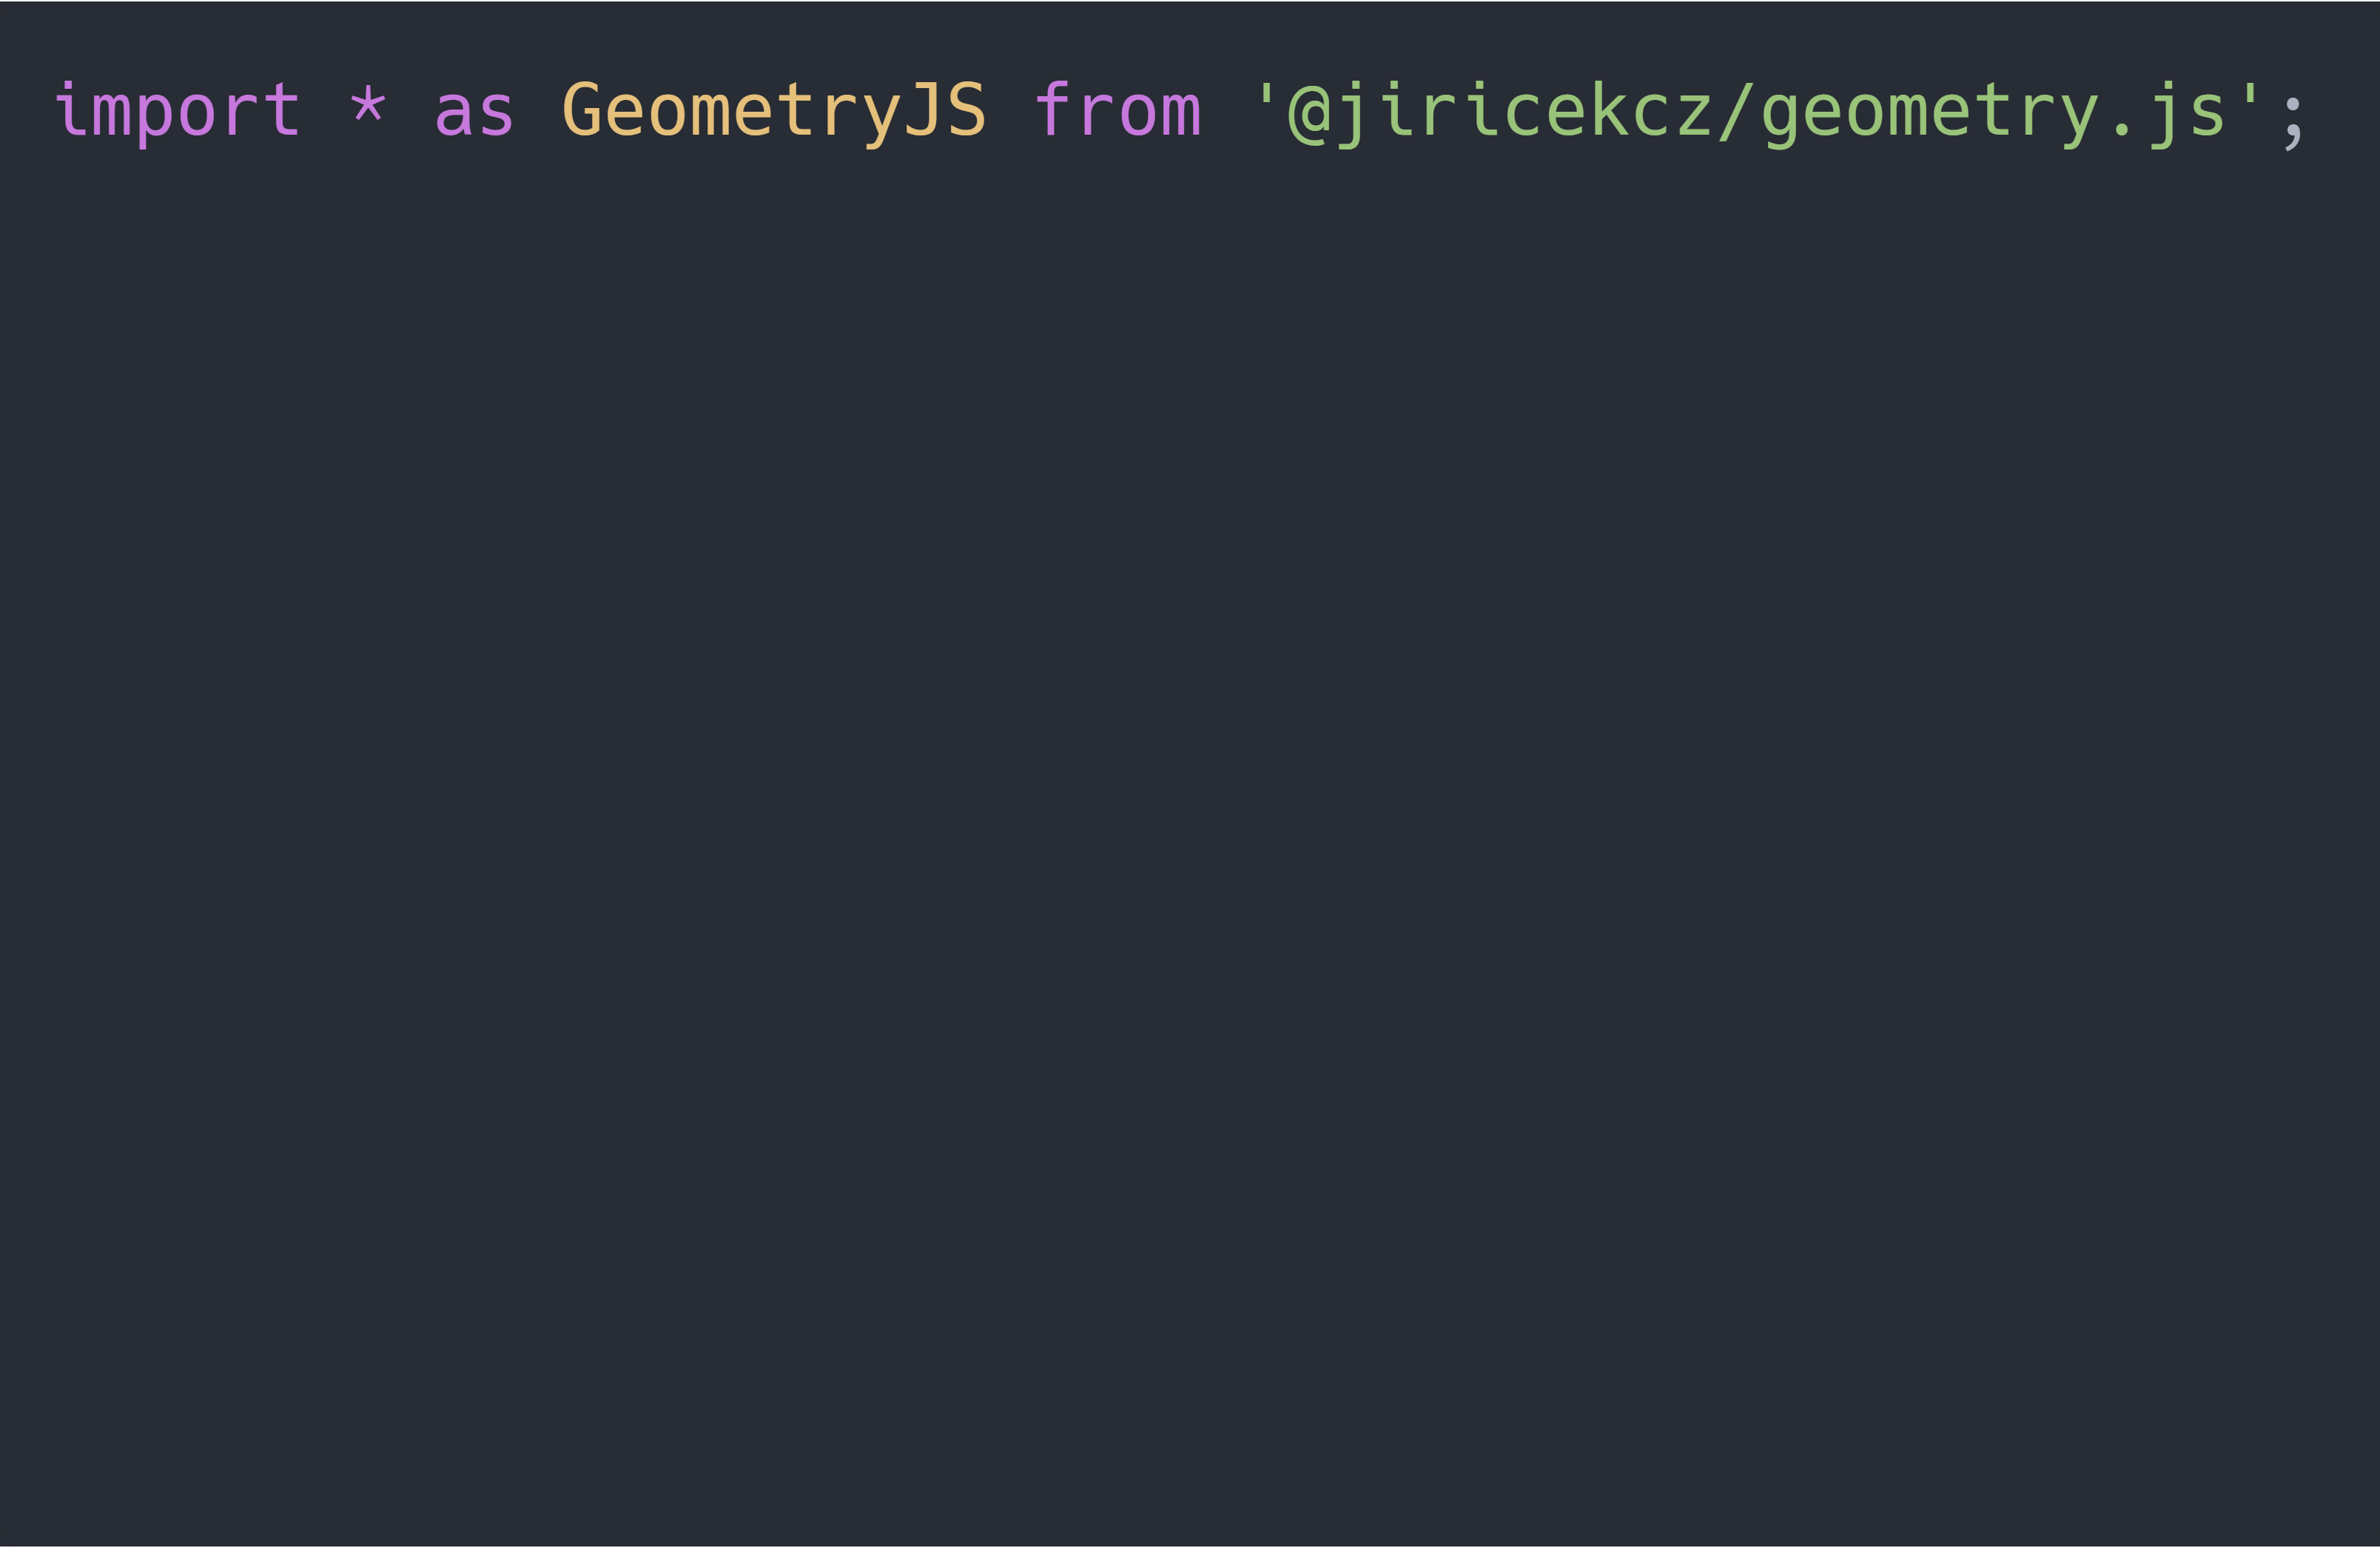
\includegraphics[height=0.715\textheight,left]{../resources/snippets/example/0.ts.png}
        }
        \only<2>{
            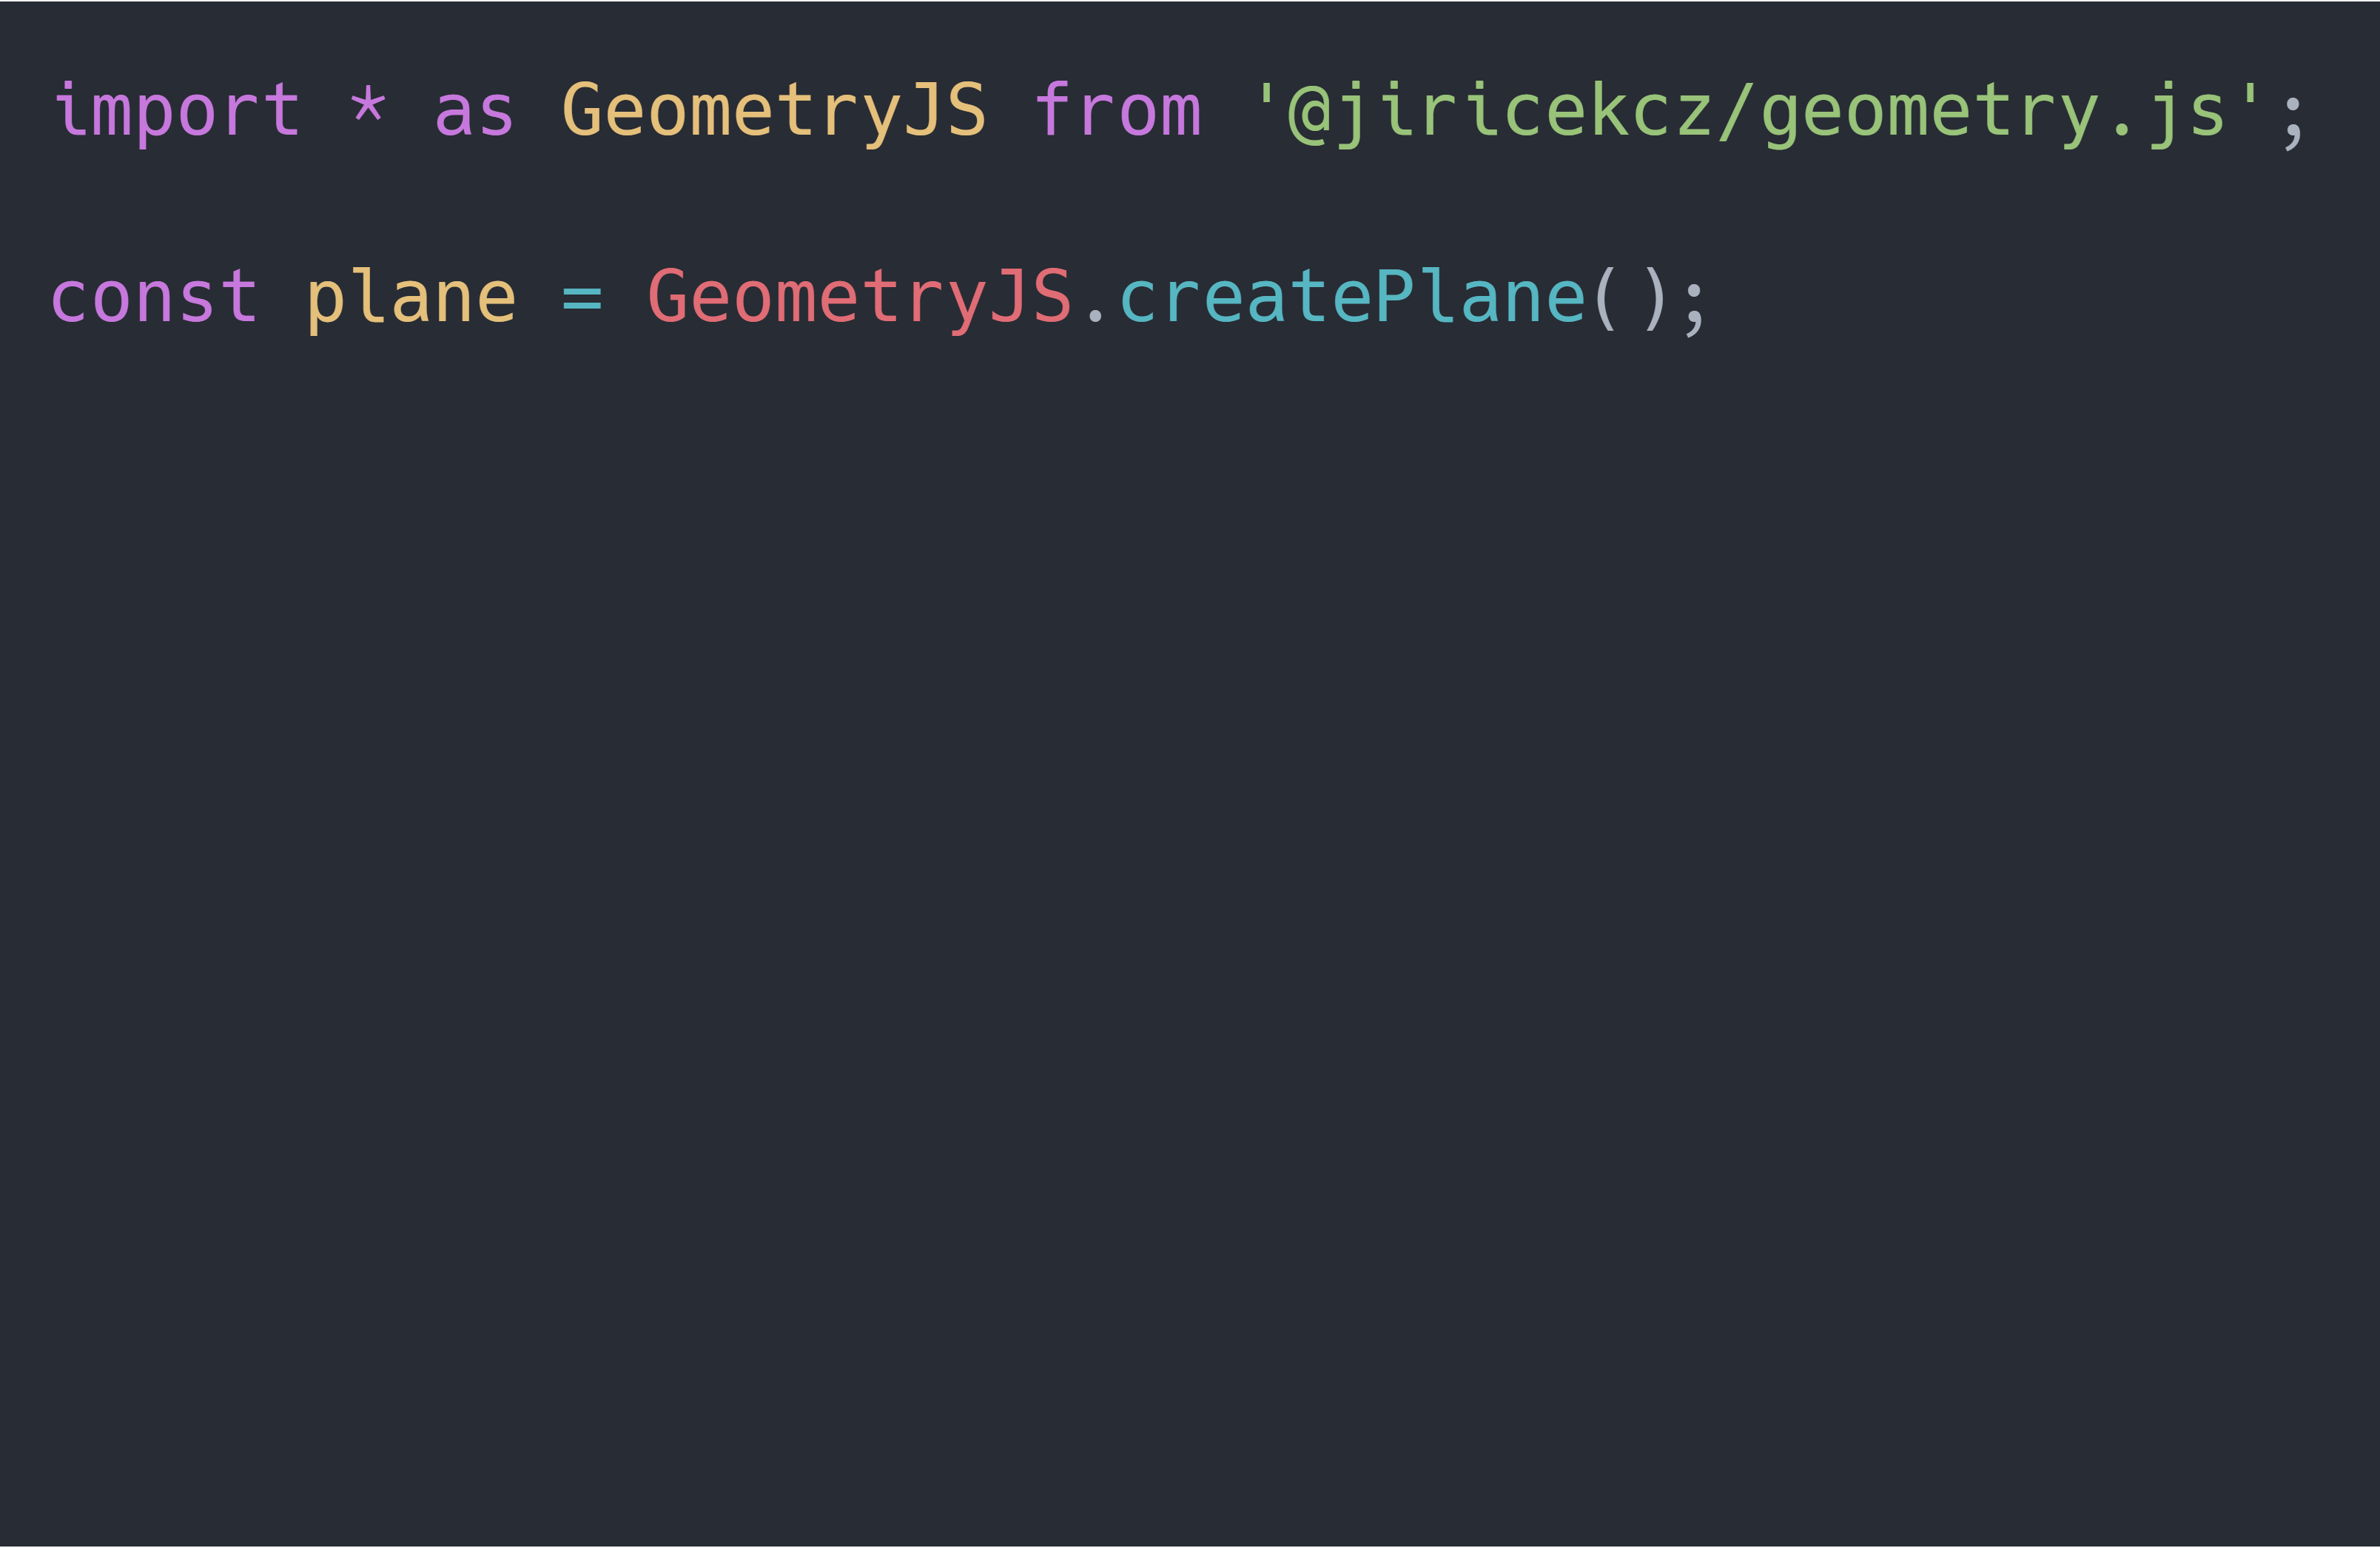
\includegraphics[height=0.715\textheight,left]{../resources/snippets/example/1.ts.png}
        }
        \only<3>{
            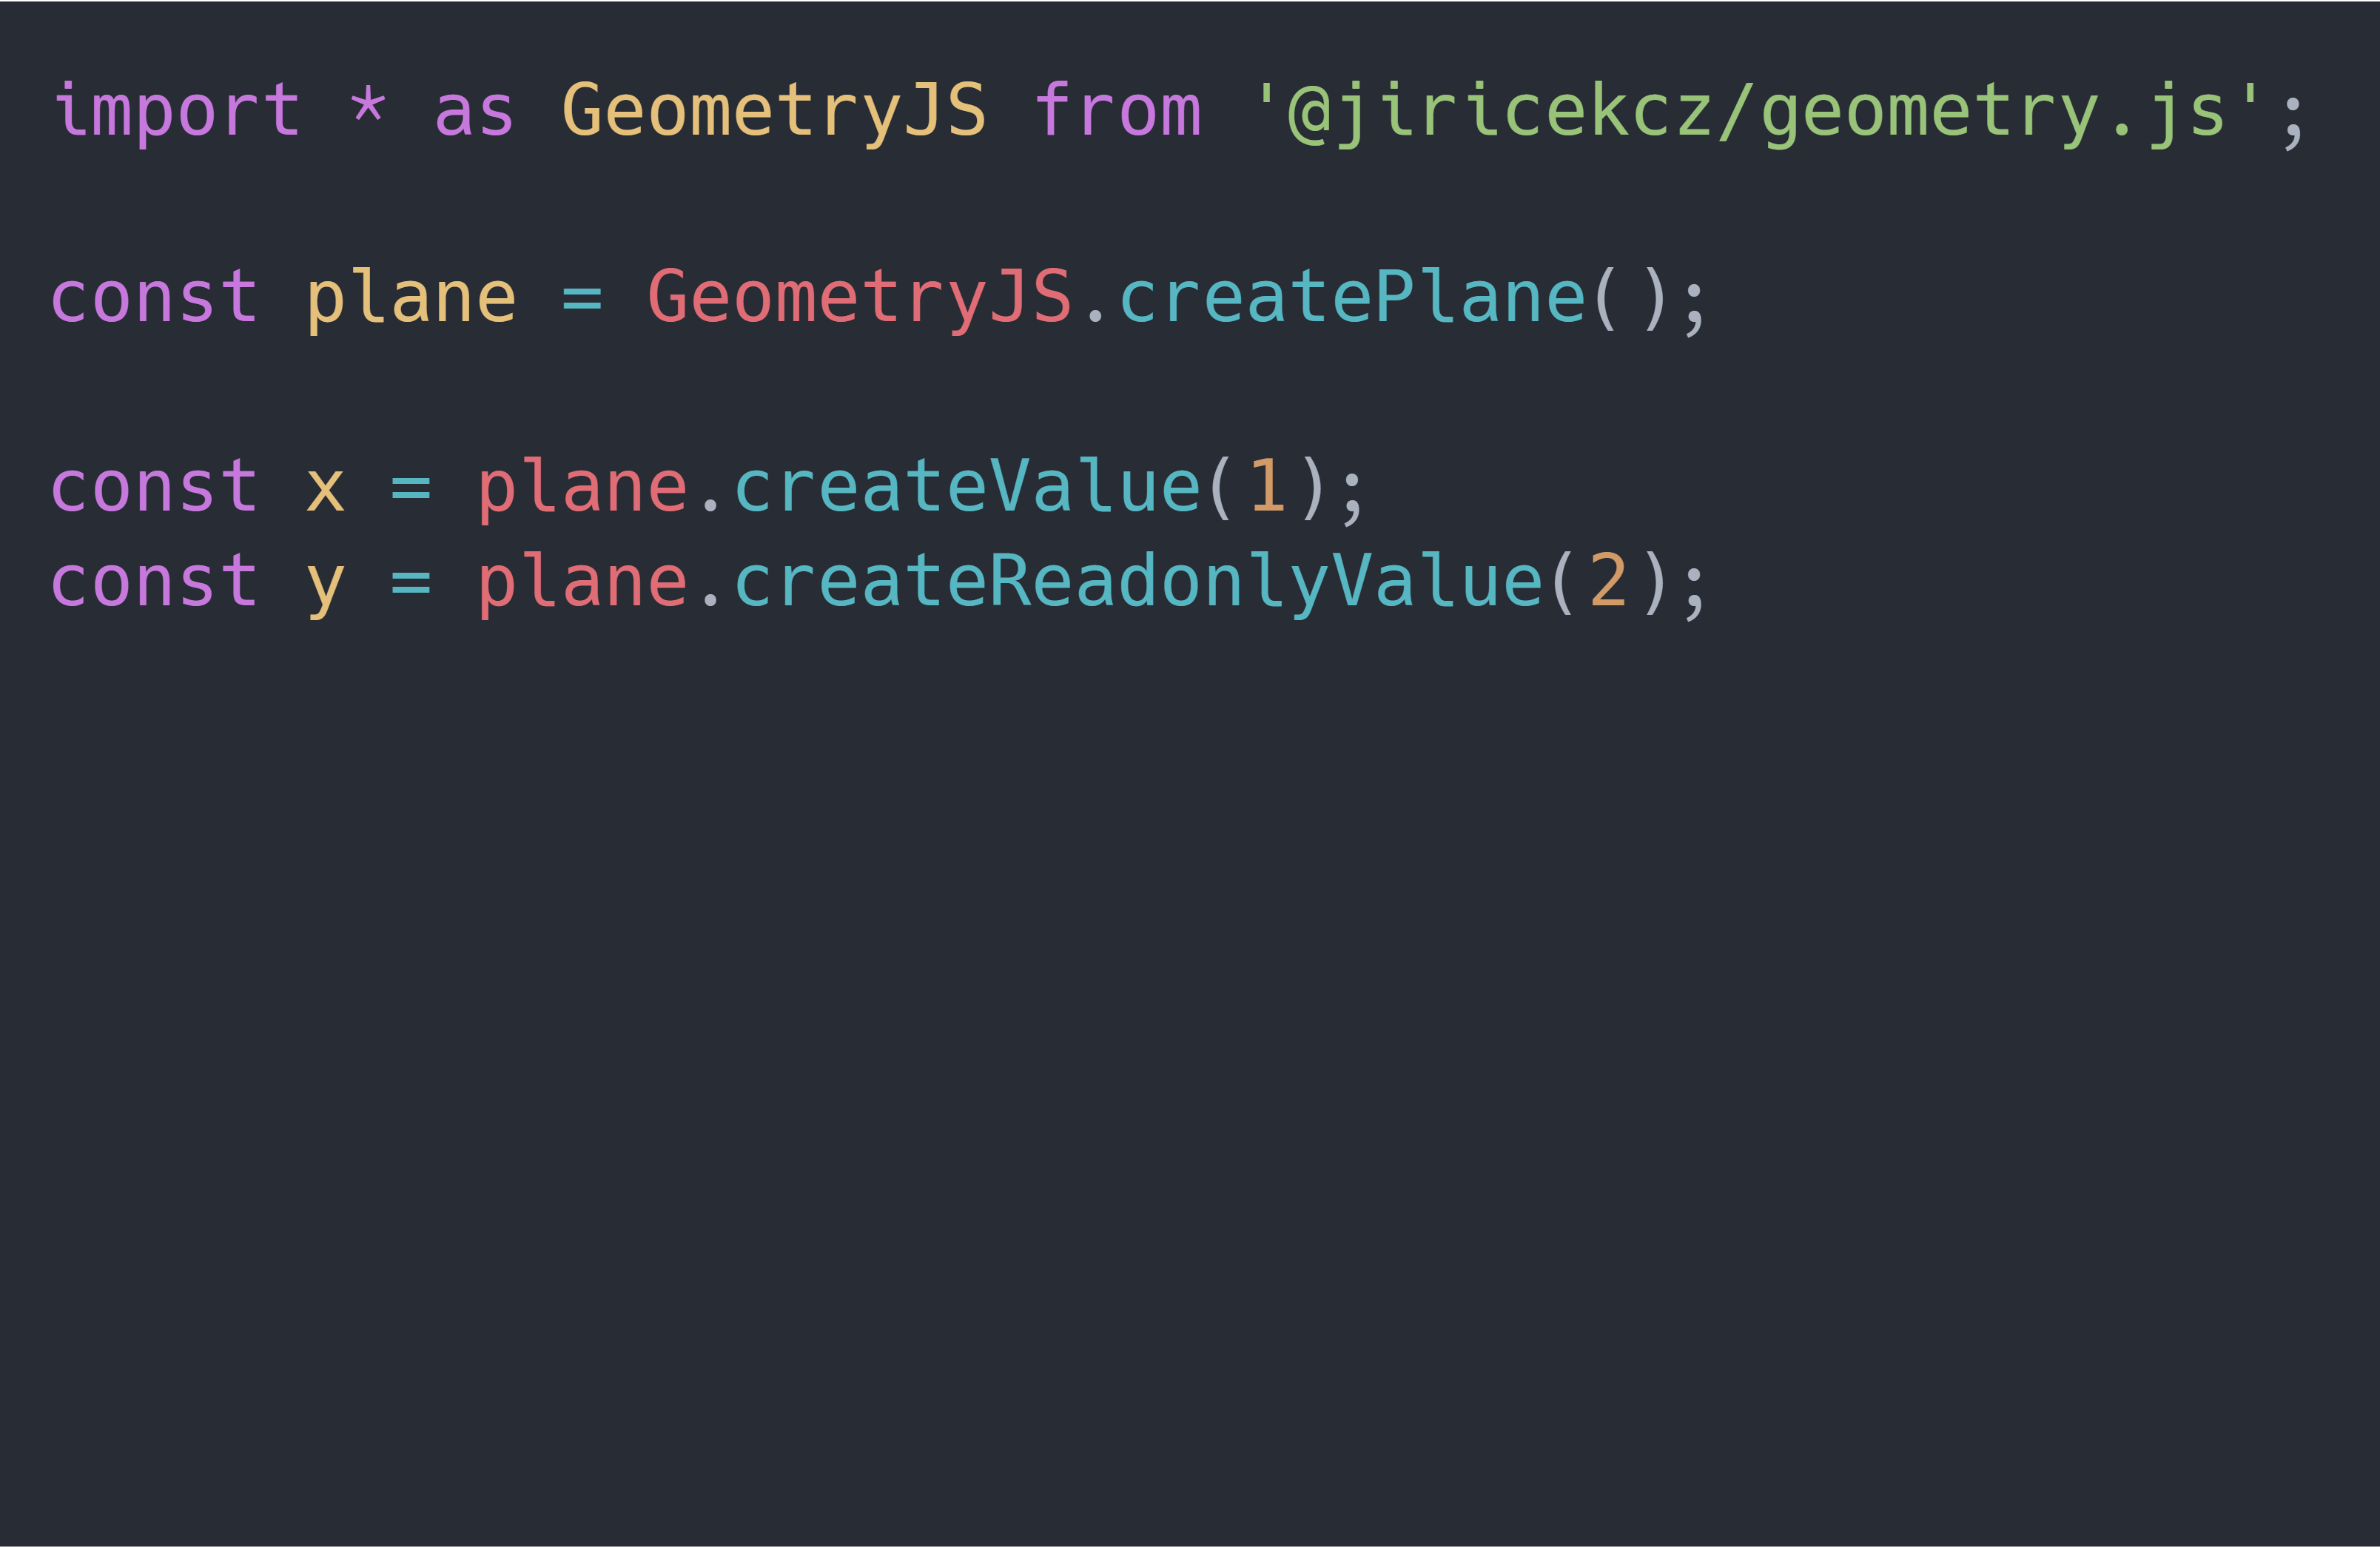
\includegraphics[height=0.715\textheight,left]{../resources/snippets/example/2.ts.png}
        }
        \only<4>{
            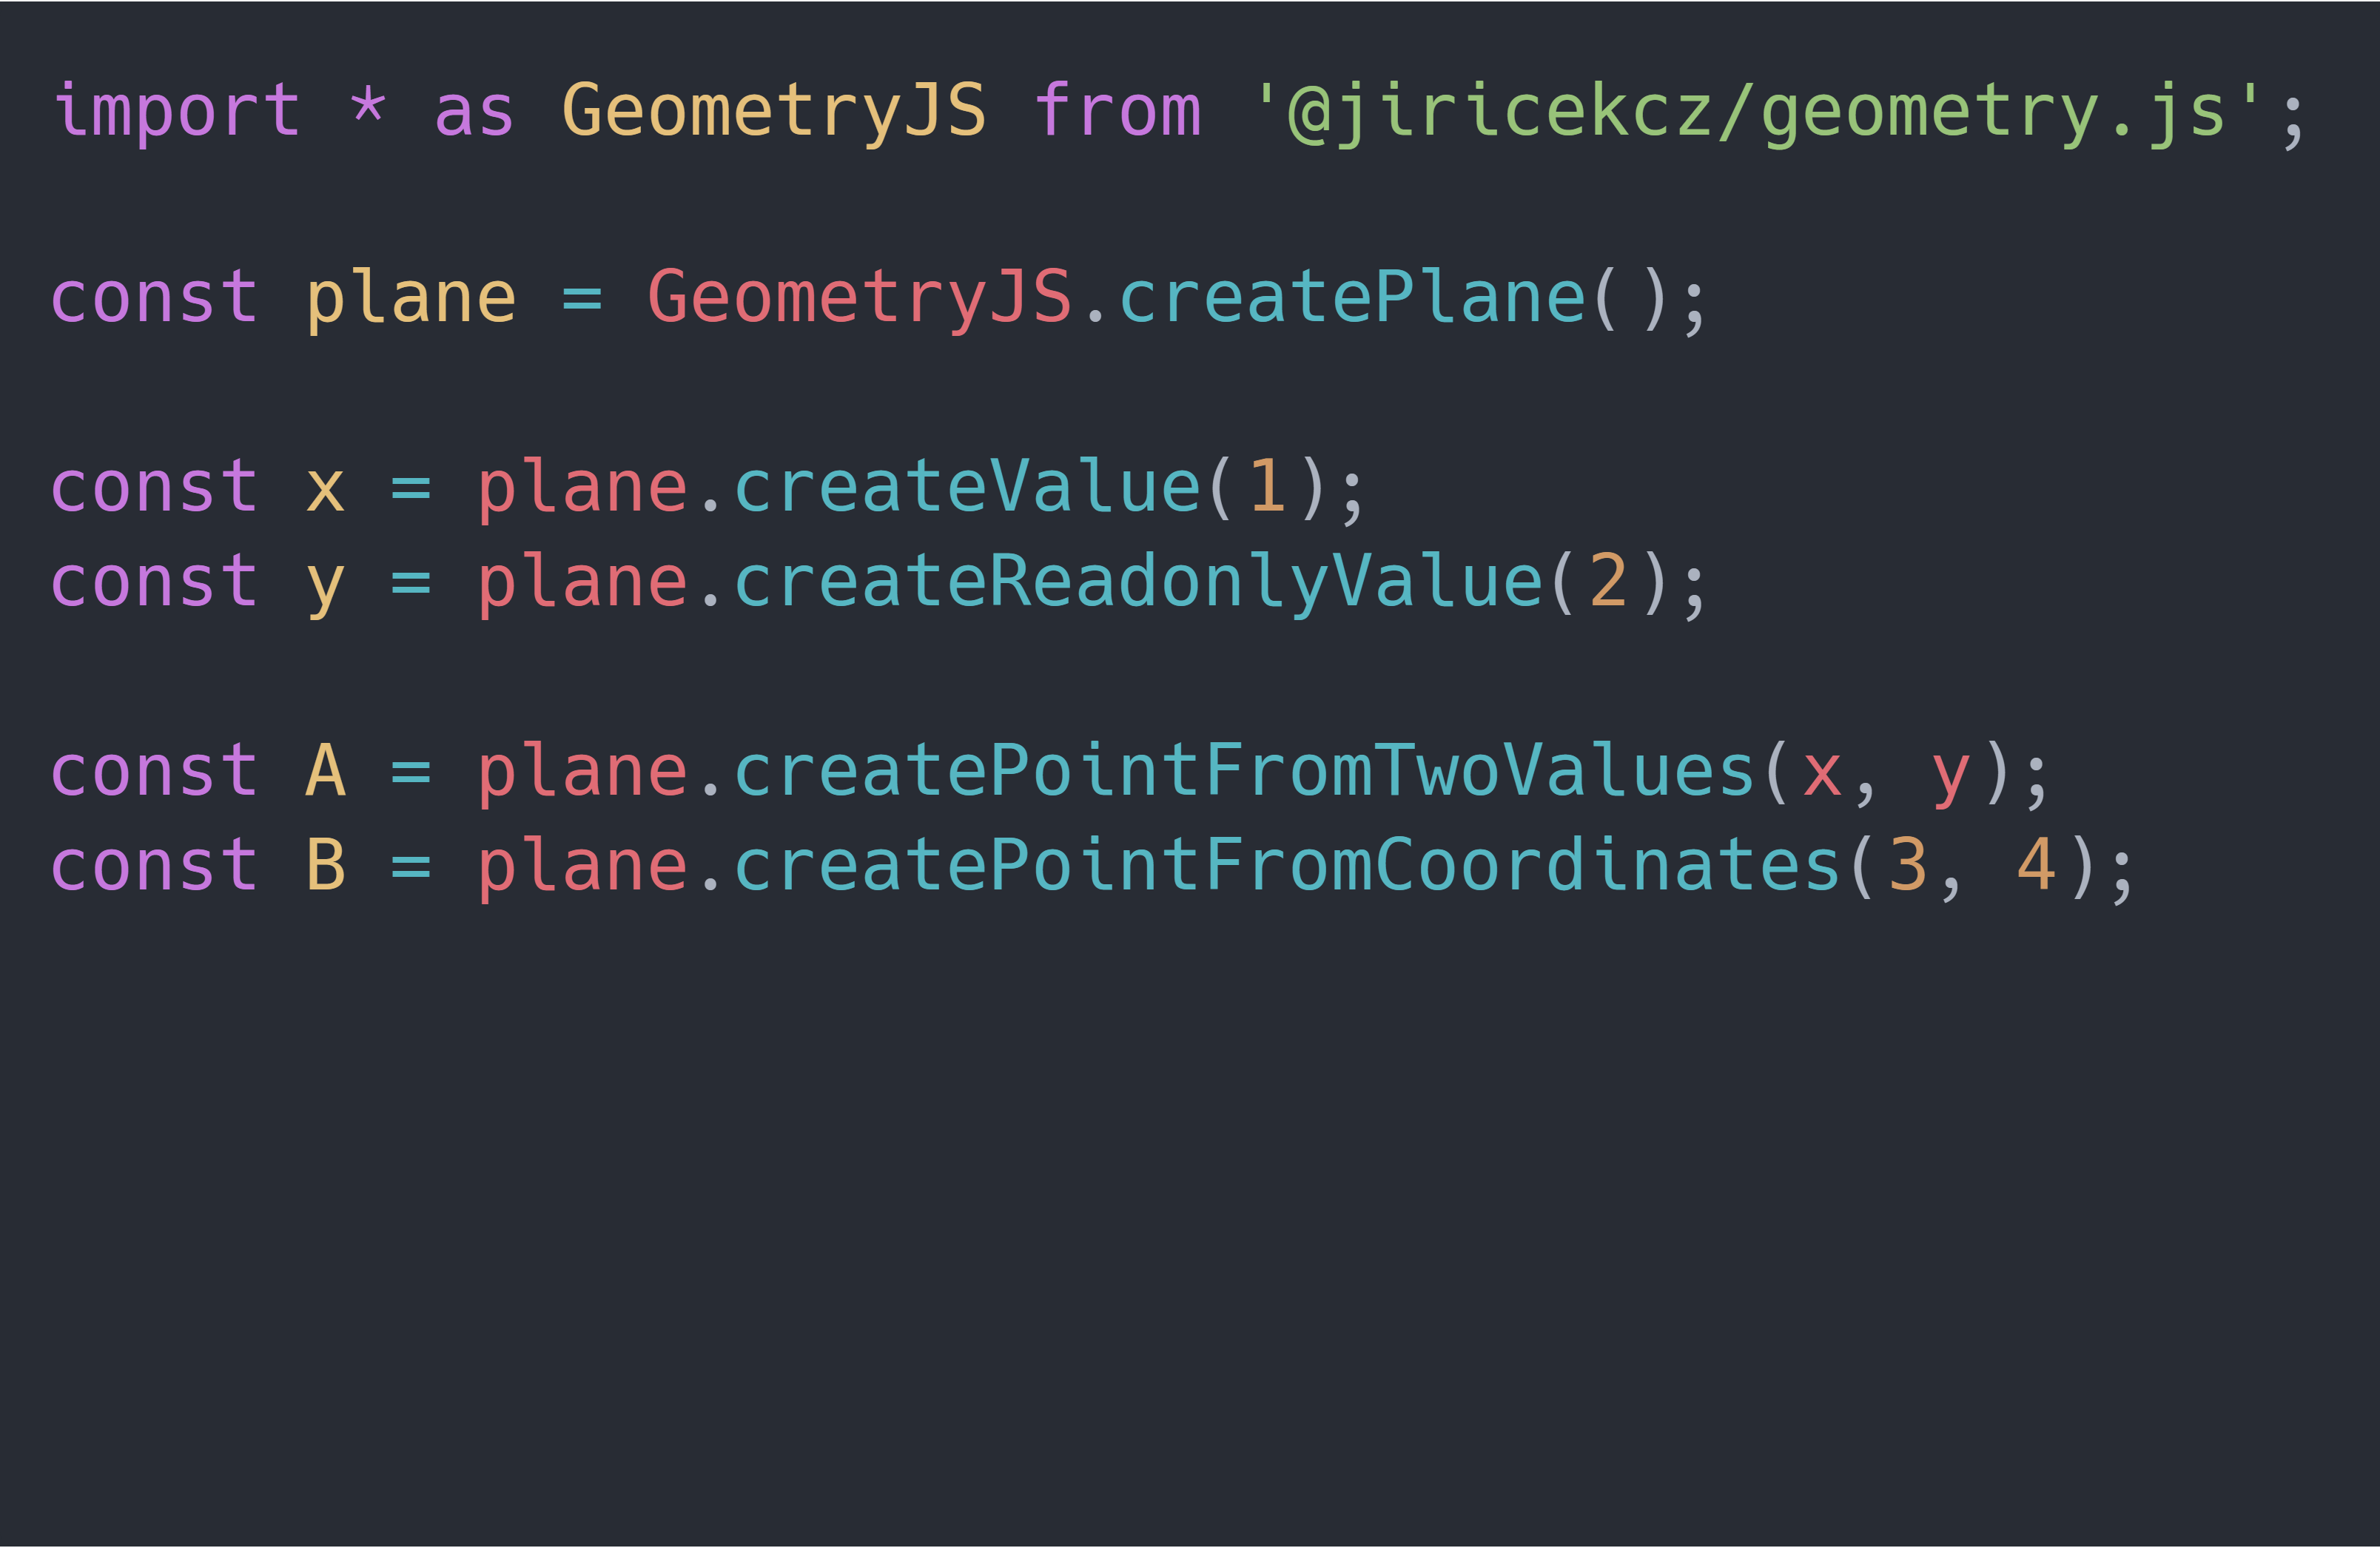
\includegraphics[height=0.715\textheight,left]{../resources/snippets/example/3.ts.png}
        }
        \only<5>{
            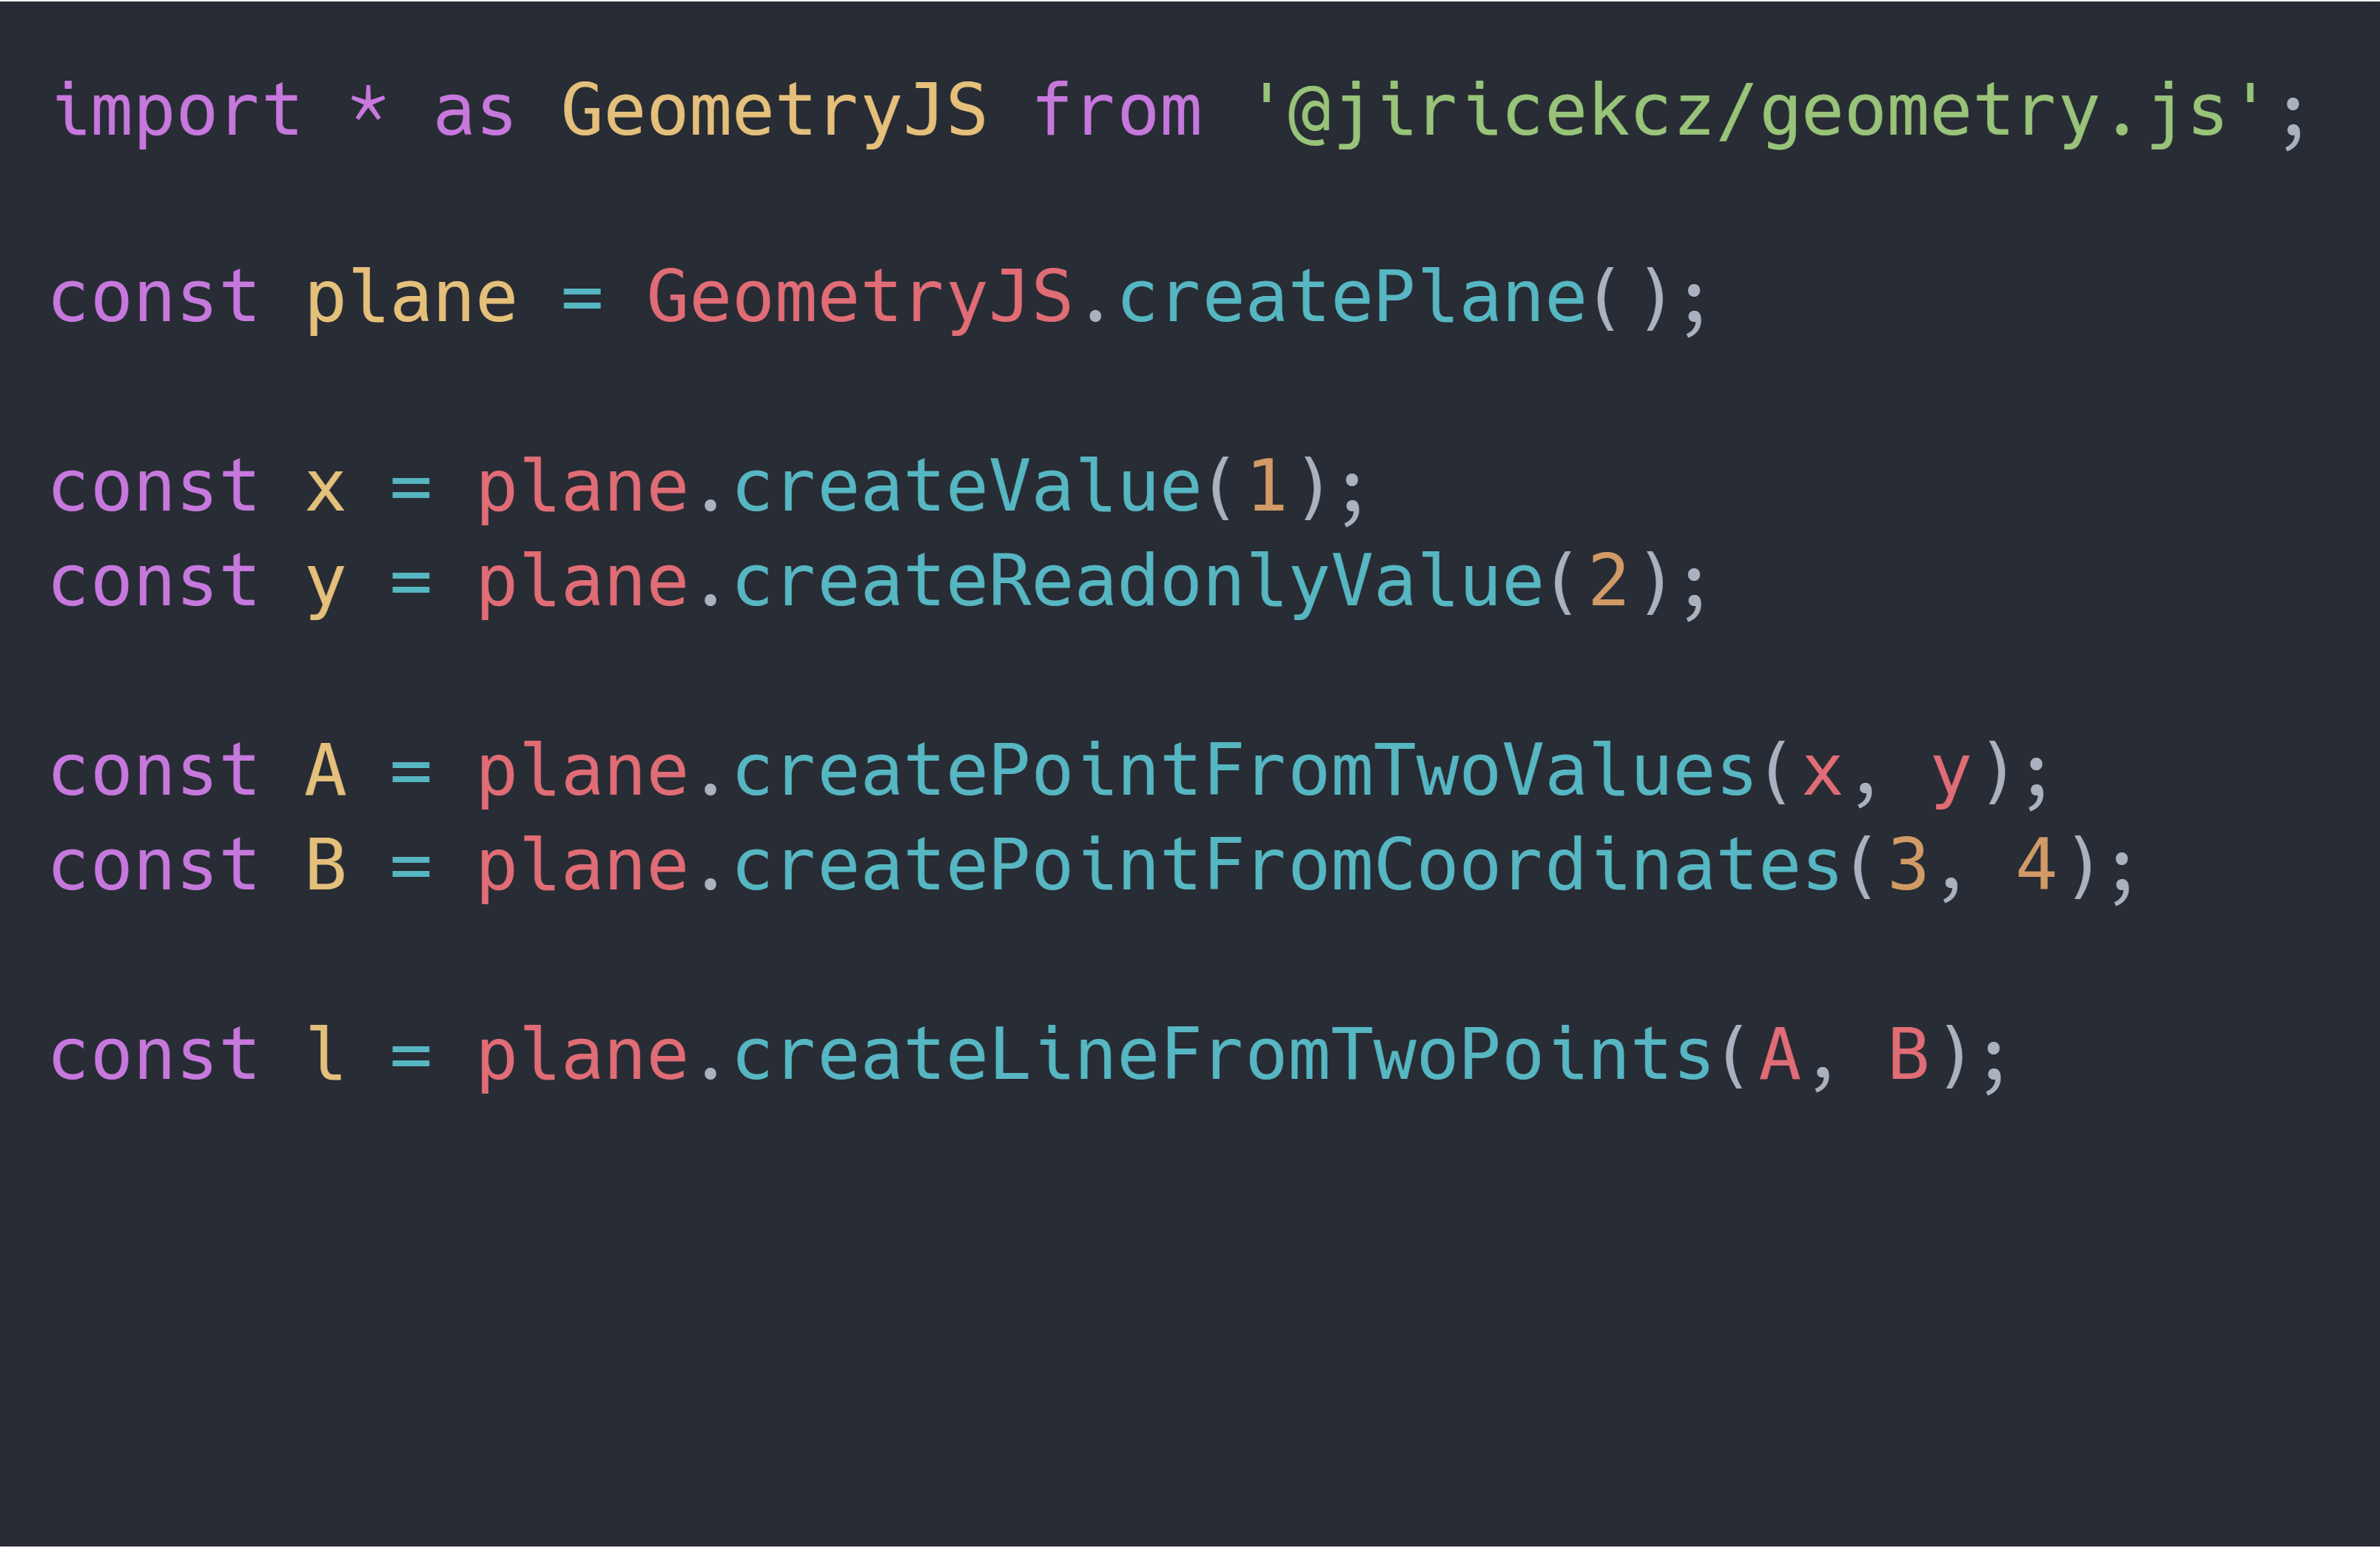
\includegraphics[height=0.715\textheight,left]{../resources/snippets/example/4.ts.png}
        }
        \only<6>{
            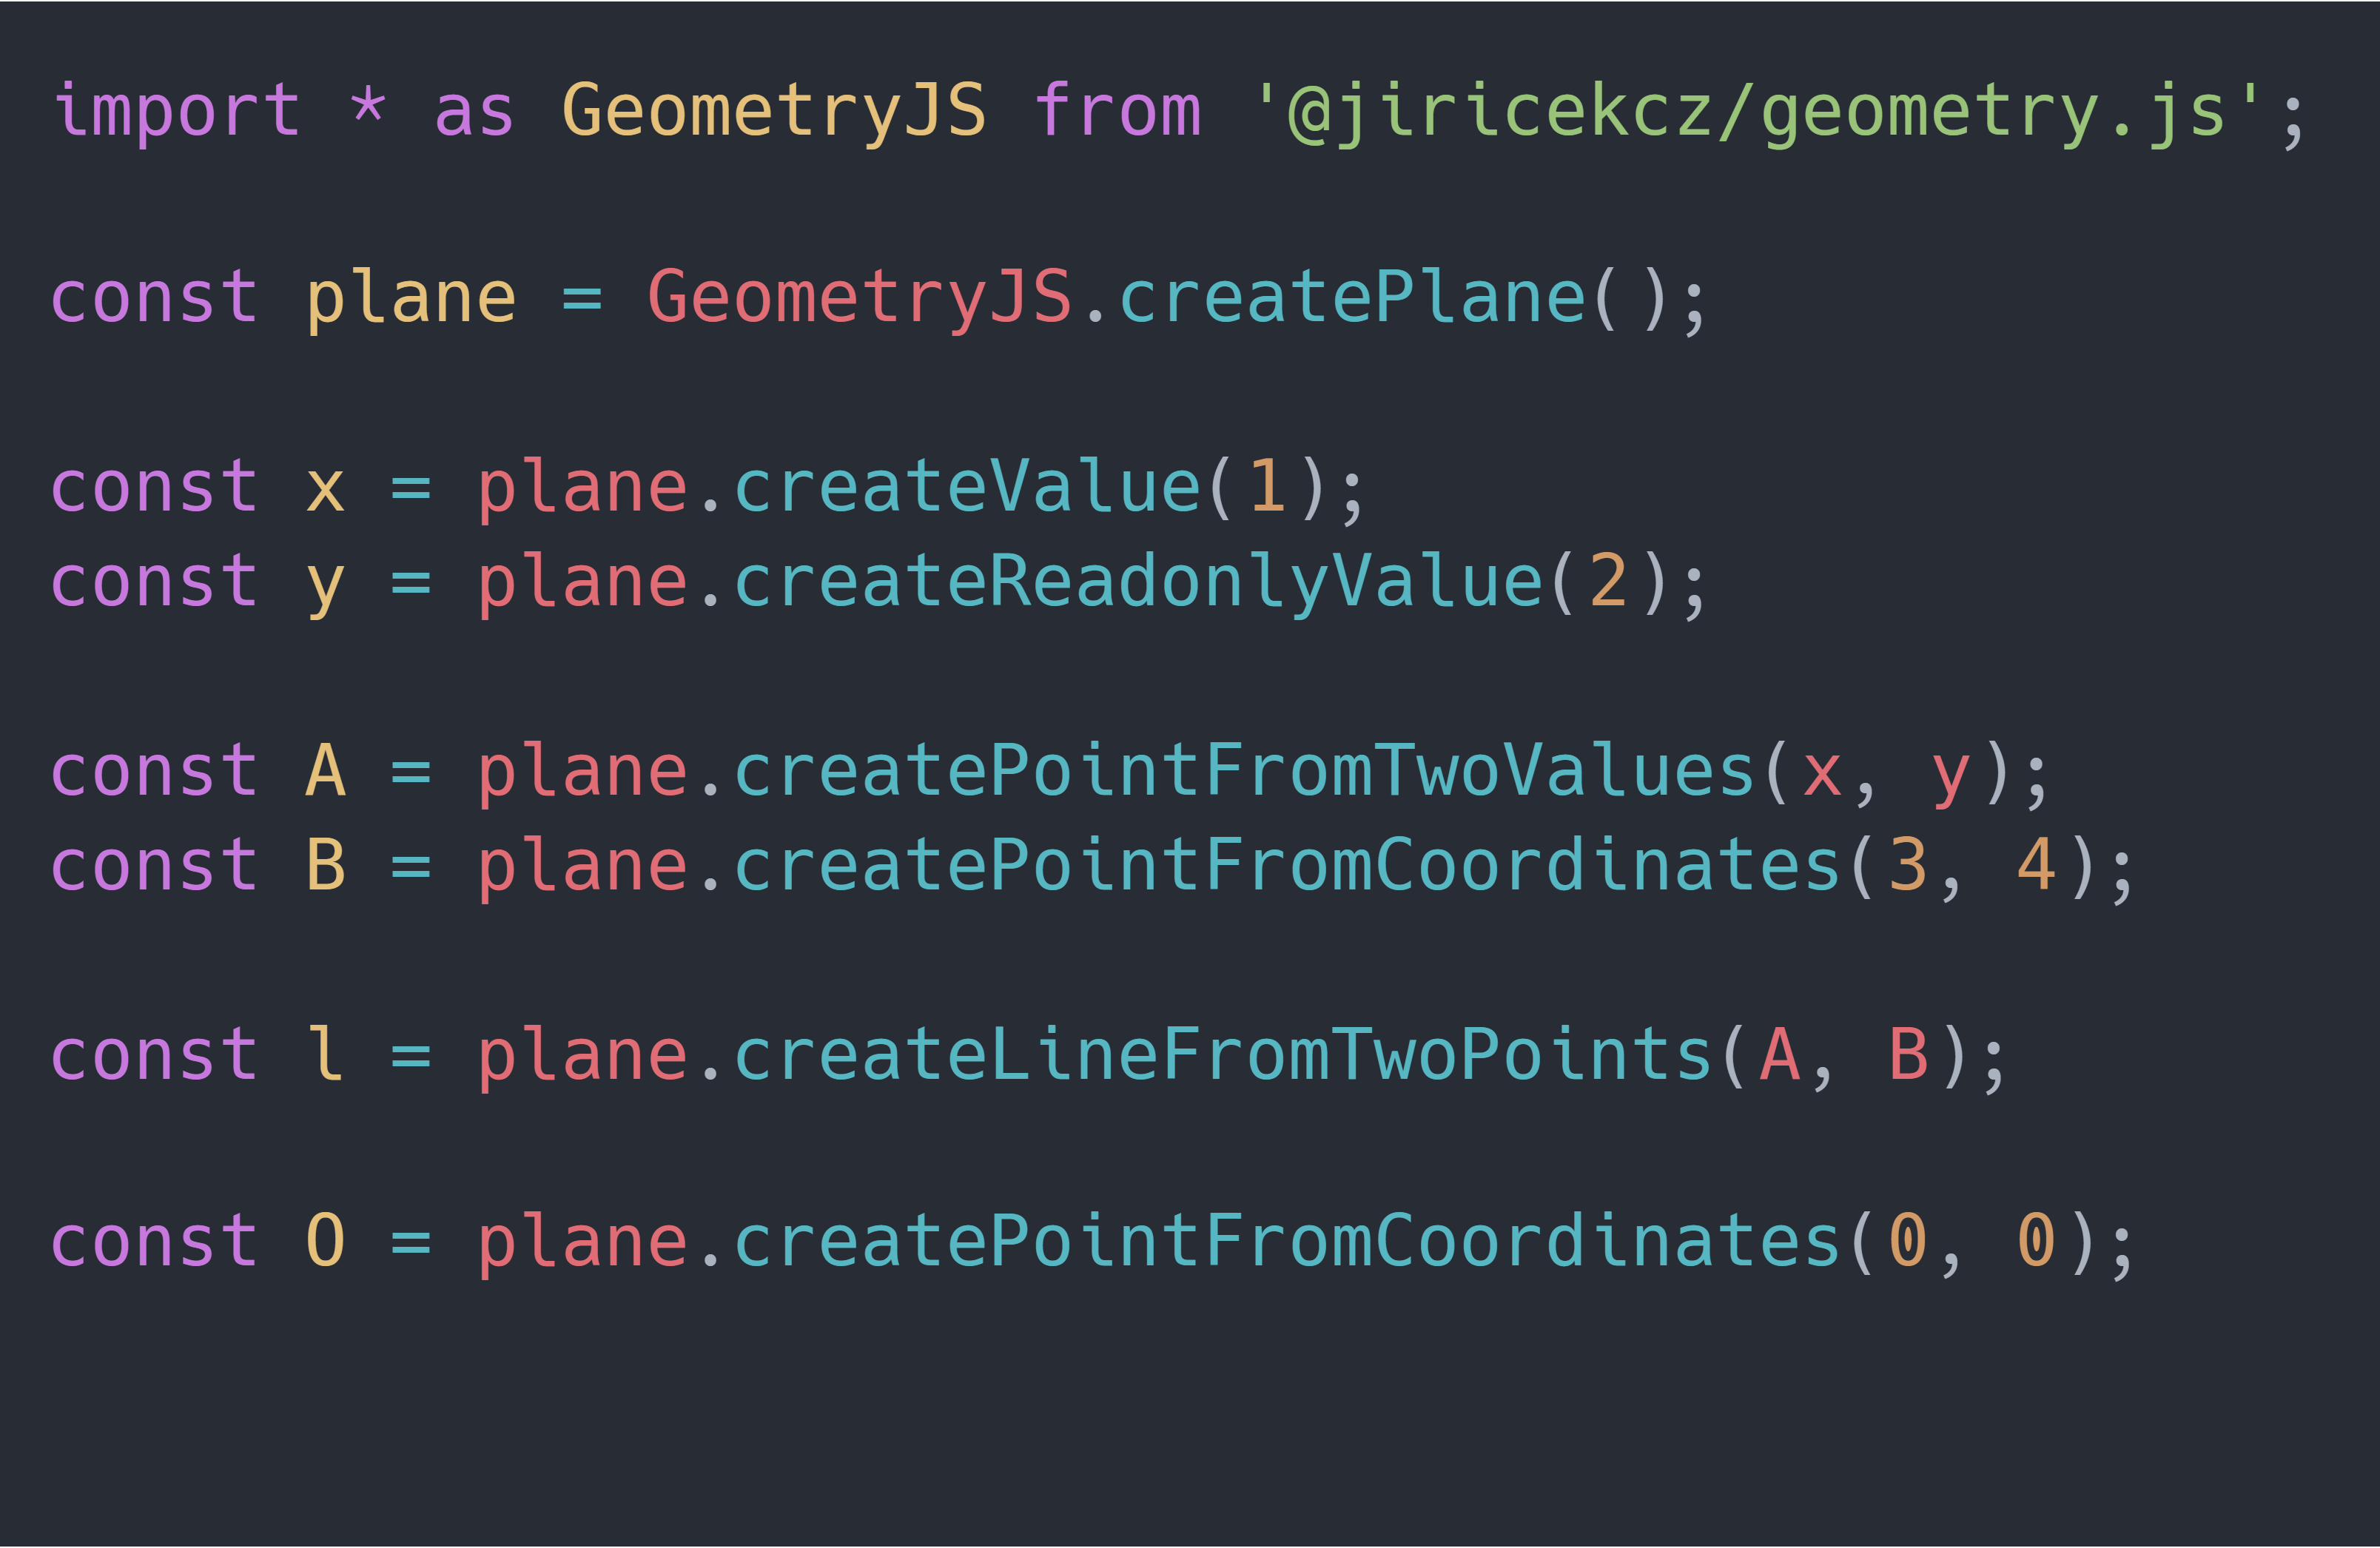
\includegraphics[height=0.715\textheight,left]{../resources/snippets/example/5.ts.png}
        }
        \only<7>{
            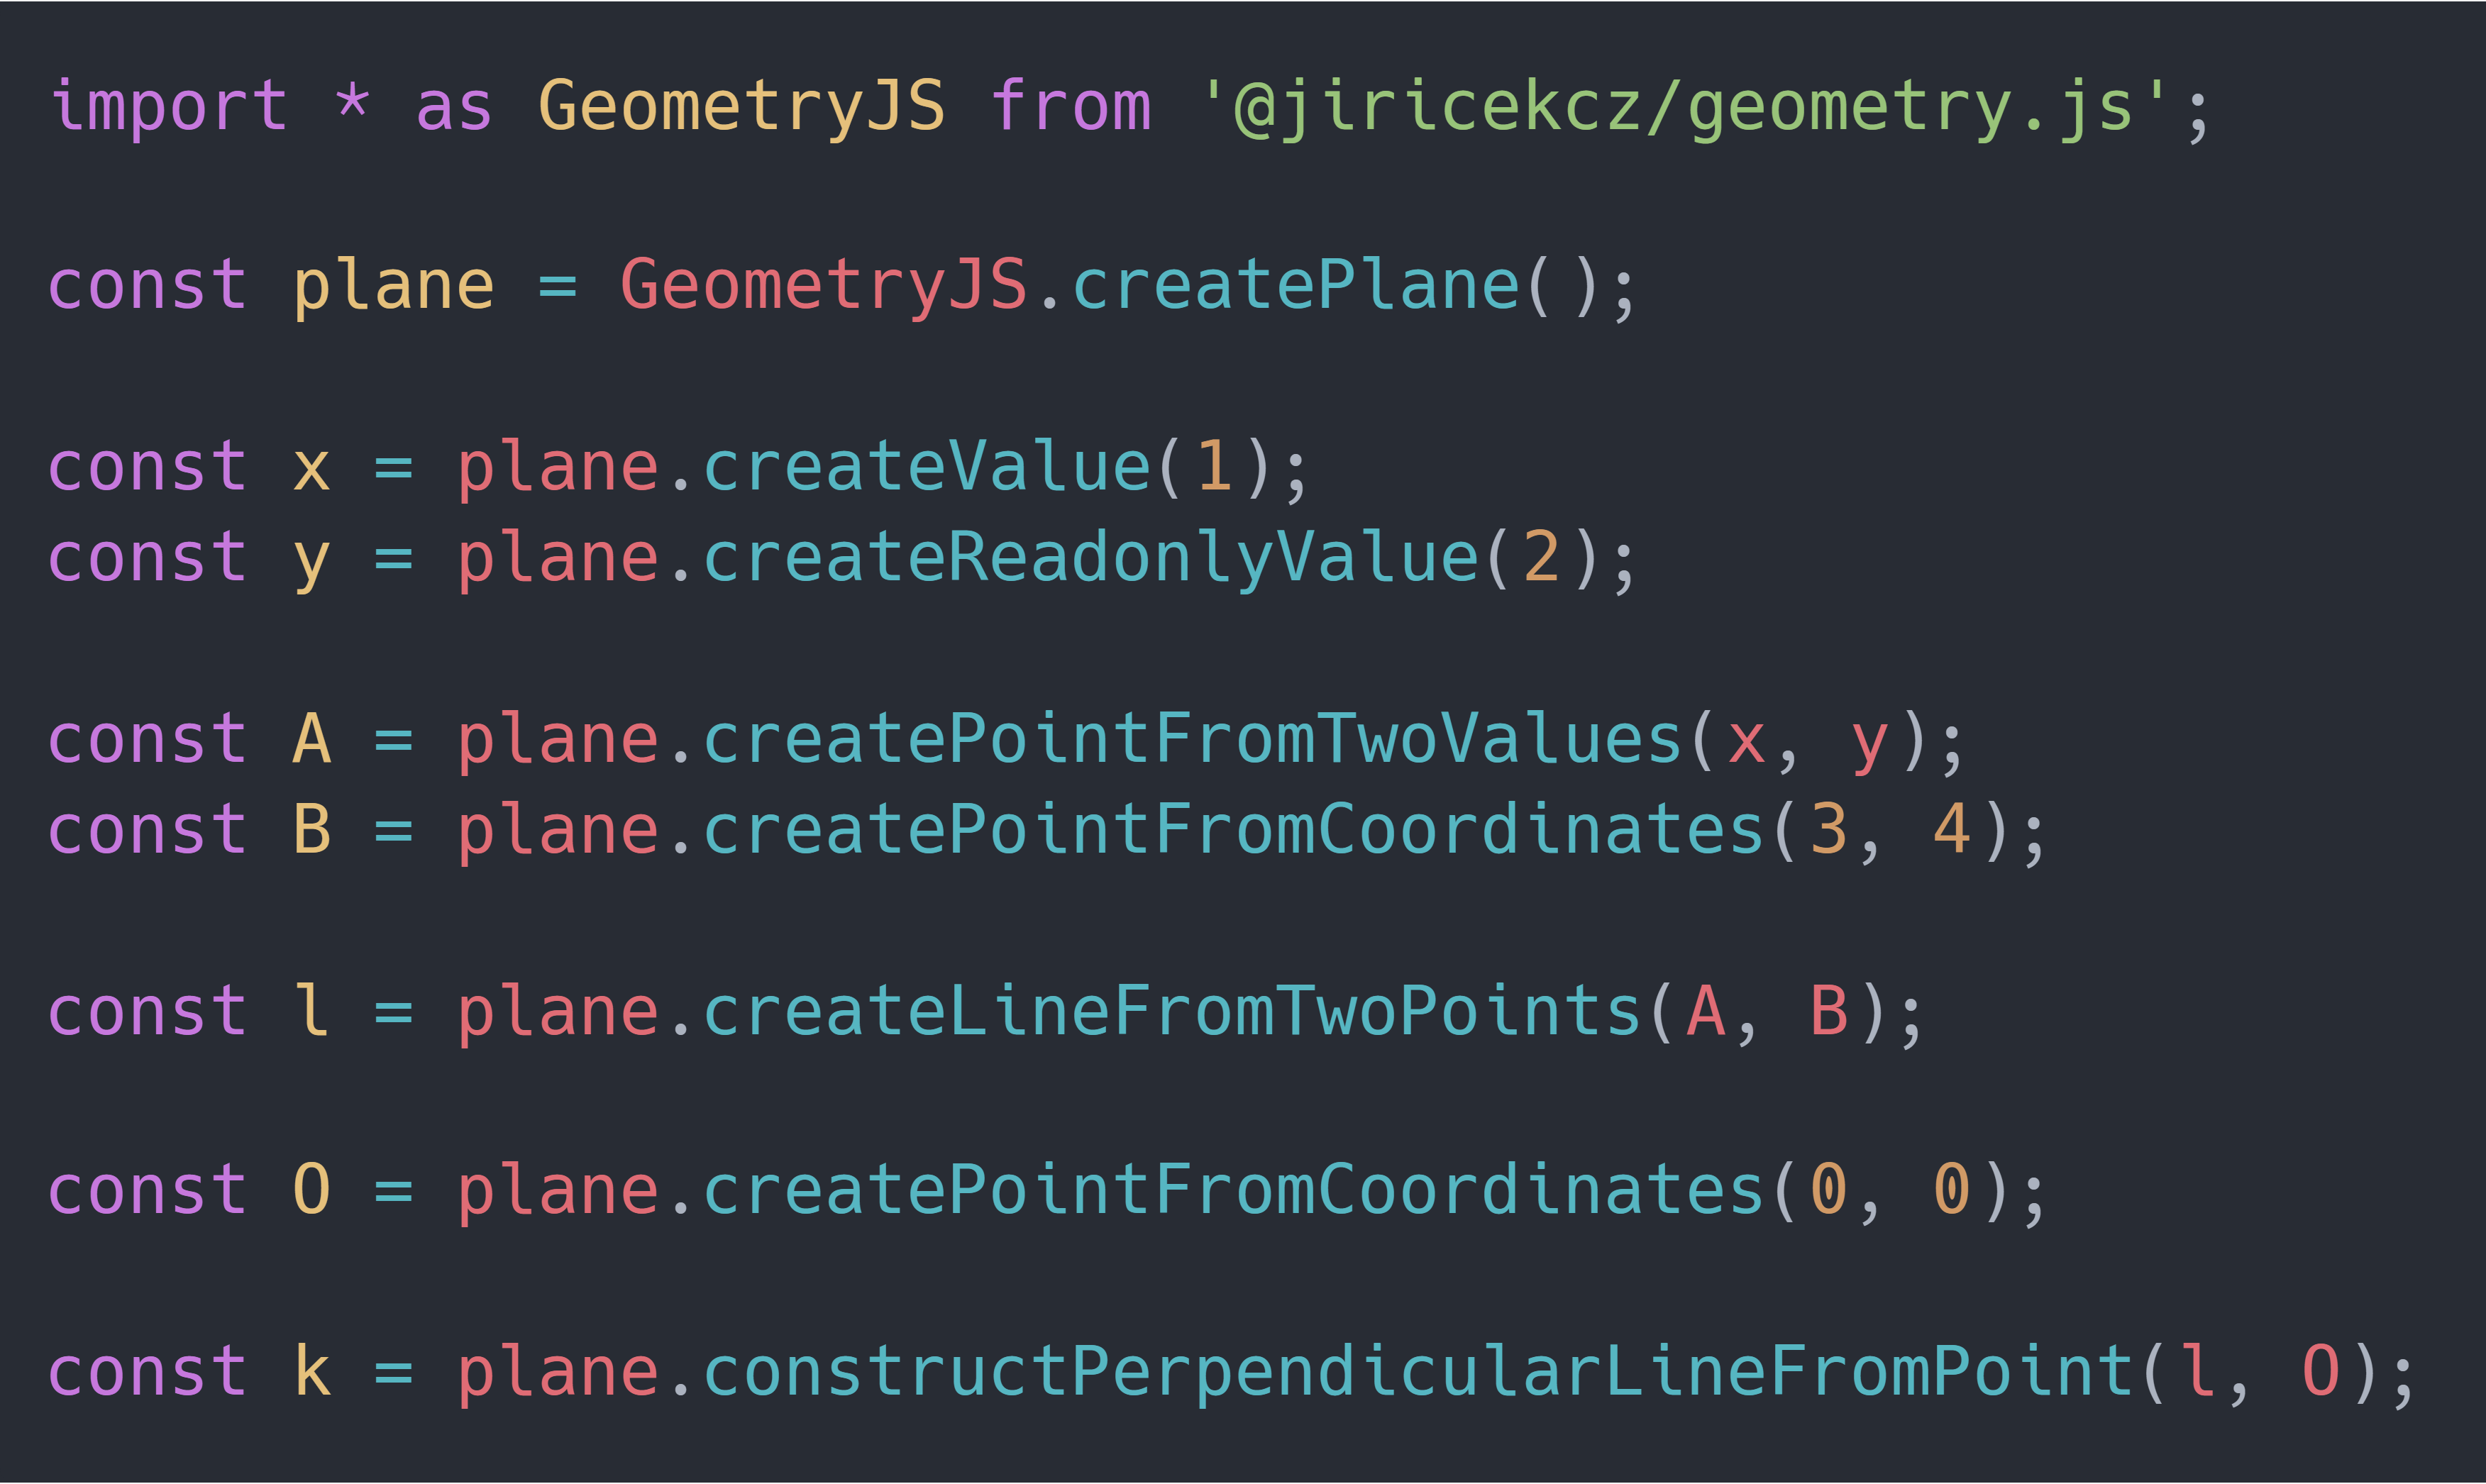
\includegraphics[height=0.715\textheight,left]{../resources/snippets/example/6.ts.png}
        }
    \end{figure}
\end{frame}